\documentclass{beamer}
\usetheme{Pittsburgh} 
%\documentclass{article}

\usepackage[utf8]{inputenc}
\usepackage{default}
%\usepackage{natbib}
\usepackage{listings}
%\usepackage{fontspec}


\begin{document}

\title{Python 2.7.6}
\subtitle{}
\author{
  Mallick, Arka\\
  Naazare, Menaka \\
  Nair, Deebul\\
  Quignon, Christophe \\
  %Familyname, Name \texttt{email}
} 
\institute{Hochschule Bonn Rhein Sieg}
\date{\today}

\begin{frame}
\titlepage
\end{frame}

%CONTENTS
%Please produce a short set of summary slides surveying the programming language concepts concerning the following topics:

%    a "Hello world" program in the language
%    a brief description of the compilation model
%    a complete list of primitive data types supported by the language
%    a description of expressions, including operator precedences
%    a list of control flow constructs, including small examples
%    a description of exception handling


%The task is to be solved in group in class.
%Produce your results in presentable form, e.g. as a set of slides.
%Put the presentation in a directory named using the following scheme: "AST-ST-2014-pl-LastNamesInAlphabeticalOrder", where you replace pl by the language you took care of and LastNames by a camel cased concatenation of the last names of your team members in alphabetical order. Then zip the directory and upload here.

\begin{frame}
\frametitle{"Hello world"}
\framesubtitle{}
 
 \begin{figure}
 \center
 %file is copyrigted
 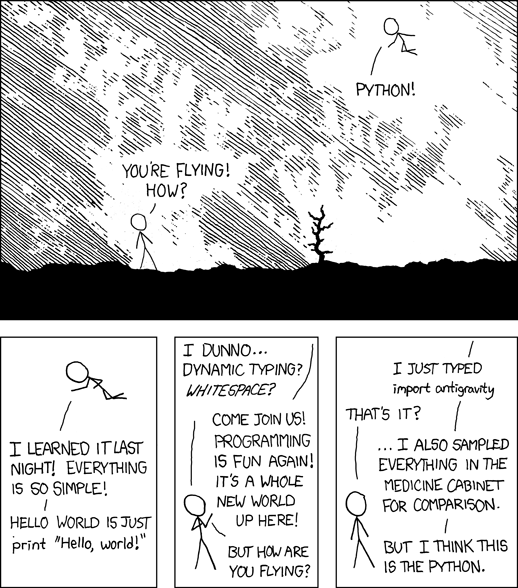
\includegraphics[width=5cm]{img/python.png}
 \caption{\href{http://xkcd.com/353/}{xkcd.com/353/}}
\end{figure}
 
\end{frame}

\begin{frame}
\frametitle{Running Python Code}
\begin{itemize}
\item Interpreter Vs Compiler

\item What happens when you execute a line of code in your python REPL?
	\begin{figure}
	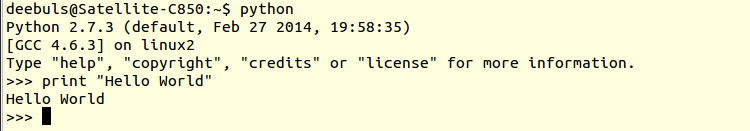
\includegraphics[width=10cm]	{Interpreter.png}
	\end{figure}
\item There are four steps that python takes when you hit return:
	\begin{itemize}
	
	\item lexing
	\item parsing
	\item compiling and 
	\item interpreting
	\end{itemize}
\end{itemize}

  
\end{frame}


\begin{frame}
\frametitle{Compiling Python Code}
Source Code is Compiled to some kind of byte code and executed by a virtual machine
\begin{itemize}
\item Cpython: Source Code -  Python byte code
	\begin{itemize}
	\item VM written in C, standard implementation
	\end{itemize}
\item Jython: Source Code - Java byte code
	\begin{itemize}
	\item JVM as runtime environment
	\end{itemize}
\item IronPython: Source Code - IL (".NET") byte code
	\begin{itemize}
	\item CLR as runtime environment
	\end{itemize}
\end{itemize}

  
\end{frame}

\begin{frame}
\frametitle{CPython Interpreter and Compiling}
	\begin{figure}
	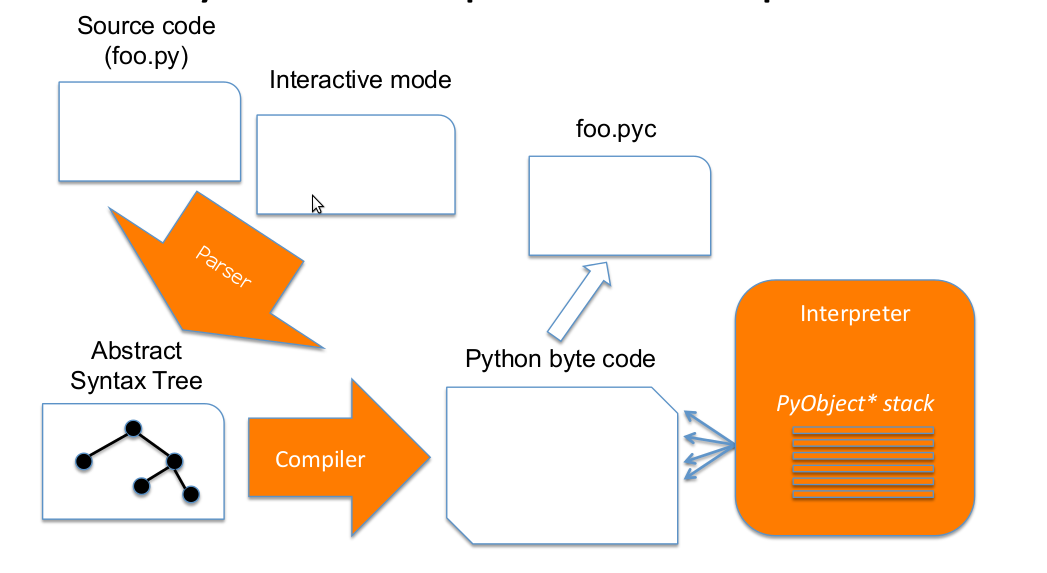
\includegraphics[width=12cm]{Cpython.png}
	\caption{\href{http://www.troeger.eu/files/teaching/pythonvm08.pdf}{CPython}}
	\end{figure}

\end{frame}
\begin{frame}
\frametitle{complete list of primitive data types}
\framesubtitle{}
  
\end{frame}

\begin{frame}
\frametitle{description of expressions}
\framesubtitle{from lowest to highest precedence}
 %CQ
 \scriptsize
 \begin{tabular}{l | l}
 \textbf{Operators} 				& \textbf{Description}\\\hline
 \texttt{lambda args: expression}		& anonymous function\\
 \texttt{if x:, else:}				& (operational precedence only)\\
 
 \texttt{x or y} 				& logical or (lazy)\\
 \texttt{x and y} 				& logical and (lazy)\\
 \texttt{not x}					& locial negation\\
 \texttt{x $<$ y, x $<=$ y, x $>$ y}		& comparison operators (value based)\\
 \texttt{x $>=$ y, x == y, x $<>$ y, x!= y}	& \\
 \texttt{x is y, x is not y}			& object identity \\
 \texttt{x in y, x not in y} 			& sequence membership\\
 
 \texttt{x \textbar y, x \^{} x, x \& y} 	& bitwise comparison\\
 \texttt{x $<<$ y, x $>>$ y} 			& left/ right shift of x by y bits\\
 
 \texttt{x + y, x - y} 				& add/concat, substract\\
 \texttt{x * y, x \% y, x / y, x // y} 	& multiply/ repeate, remainder/ format, division\\
 
 \texttt{-x, +x, \~{}x, x ** y} 		& unary negation, identity\\
						& bitwise complement, binary power\\
 
 \texttt{x[i], x[i:j], x.attr, x(\dots)} 	& indexing, slicing, qualification, function calls\\
 \texttt{(\dots), [\dots], \{\dots\}, '\dots'} & tuple, list, dictionary, string\\
 
 %left to right if two functions have the same precedence
 % except ** | 2 ** 2 ** 2 ** 2 = 65536
 % 3 < 4 < True ==  (3<4)and(4 < True)
 % x = 1
 % y = x = 2
 % '1' in '11' == True
 % The if/else expression is an expression, but assignment is a statement

 \end{tabular}
\end{frame}
 

\begin{frame}
\frametitle{list of control flow constructs, including small examples}
\framesubtitle{}
%
%if, elif and else statements
%Syntax : if option 1 Condition :
%            ....
%         elif option 2 Condition :
 %           ....
%         else :
%            .... default choice   
%
%for loop
%Syntax : for iterator_name in iterating_sequence :
               statements
               ...
while loop
Syntax : While Condition :
            statements 

pass, break and continue
pass - used for the sake of syntactical correctness
continue - to continue to next iteration without doing anything to the loop.
break - to terminate the loop
\end{frame}

\begin{frame}
\frametitle{Exception Handling}
\framesubtitle{Basics}
Events that can modify the flow of control through a program.
In python, exceptions are triggered automatically on errors. It can also be both triggered and intercepted from the code. They are processed by three statements which has two variations:
\begin{itemize}
\item try/except
	\begin{itemize}
	\item Catch and recover from exceptions raised by python, or by user
	\end{itemize}
\item try/finally
	\begin{itemize}
	\item Perform cleanup actions wheter exceptions occur or not.
	\end{itemize}
\item raise
	\begin{itemize}
	\item Trigger an exception manually in your code.
	\end{itemize}
\item assert
	\begin{itemize}
	\item Conditionally trigger an exception in your code.
	\end{itemize}
\end{itemize}
  
\end{frame}


%\begin{frame}
%        \frametitle{Reference}
%        \bibliographystyle{amsalpha}%amsalpha
%        \bibliography{precoursebib.bib} 
%\end{frame}


%\begin{lstlisting}[language=Python]

%http://interactivepython.org
%http://xkcd.com/353/

\begin{frame}
 \frametitle{references}
 \begin{itemize}
  \item Mark Lutz. 2003. Learning Python (2 ed.). O'Reilly \& Associates, Inc., Sebastopol, CA, USA.
  \item \href{https://docs.python.org/2.7/}{docs.python.org/2.7/}
  \item \href{http://interactivepython.org}{interactivepython.org}
 \end{itemize}
\end{frame}


\end{document}
